\documentclass[11pt,a4paper,landscape]{article}
\usepackage[margin=10mm]{geometry}
\usepackage{graphicx}
\usepackage{tikz}
\usetikzlibrary{arrows.meta,positioning,fit,backgrounds}
\usepackage{array}
\usepackage{xcolor}
\pagestyle{empty}

\definecolor{inputblue}{RGB}{222,238,255}
\definecolor{processgreen}{RGB}{225,244,232}
\definecolor{branchyellow}{RGB}{255,245,210}
\definecolor{outputred}{RGB}{255,230,230}
\definecolor{notegrey}{RGB}{244,244,244}

\tikzset{
  box/.style={
    draw,
    rounded corners=2pt,
    align=center,
    minimum height=9mm,
    text width=34mm,
    font=\scriptsize,
    inner sep=3pt
  },
  widebox/.style={
    box,
    text width=48mm
  },
  smallbox/.style={
    box,
    text width=28mm
  },
  input/.style={box, fill=inputblue},
  process/.style={box, fill=processgreen},
  branch/.style={box, fill=branchyellow},
  output/.style={box, fill=outputred},
  note/.style={box, fill=notegrey},
  arrow/.style={-{Latex[length=2.1mm]}, thick},
  lightarrow/.style={-{Latex[length=1.8mm]}, thin},
}

\begin{document}

\begin{center}
\Large\bfseries Mie Multi-Hole Pipeline: Video to 1D Per-Frame Metrics
\end{center}

\vspace{-1mm}

\noindent\resizebox{0.95\linewidth}{!}{%
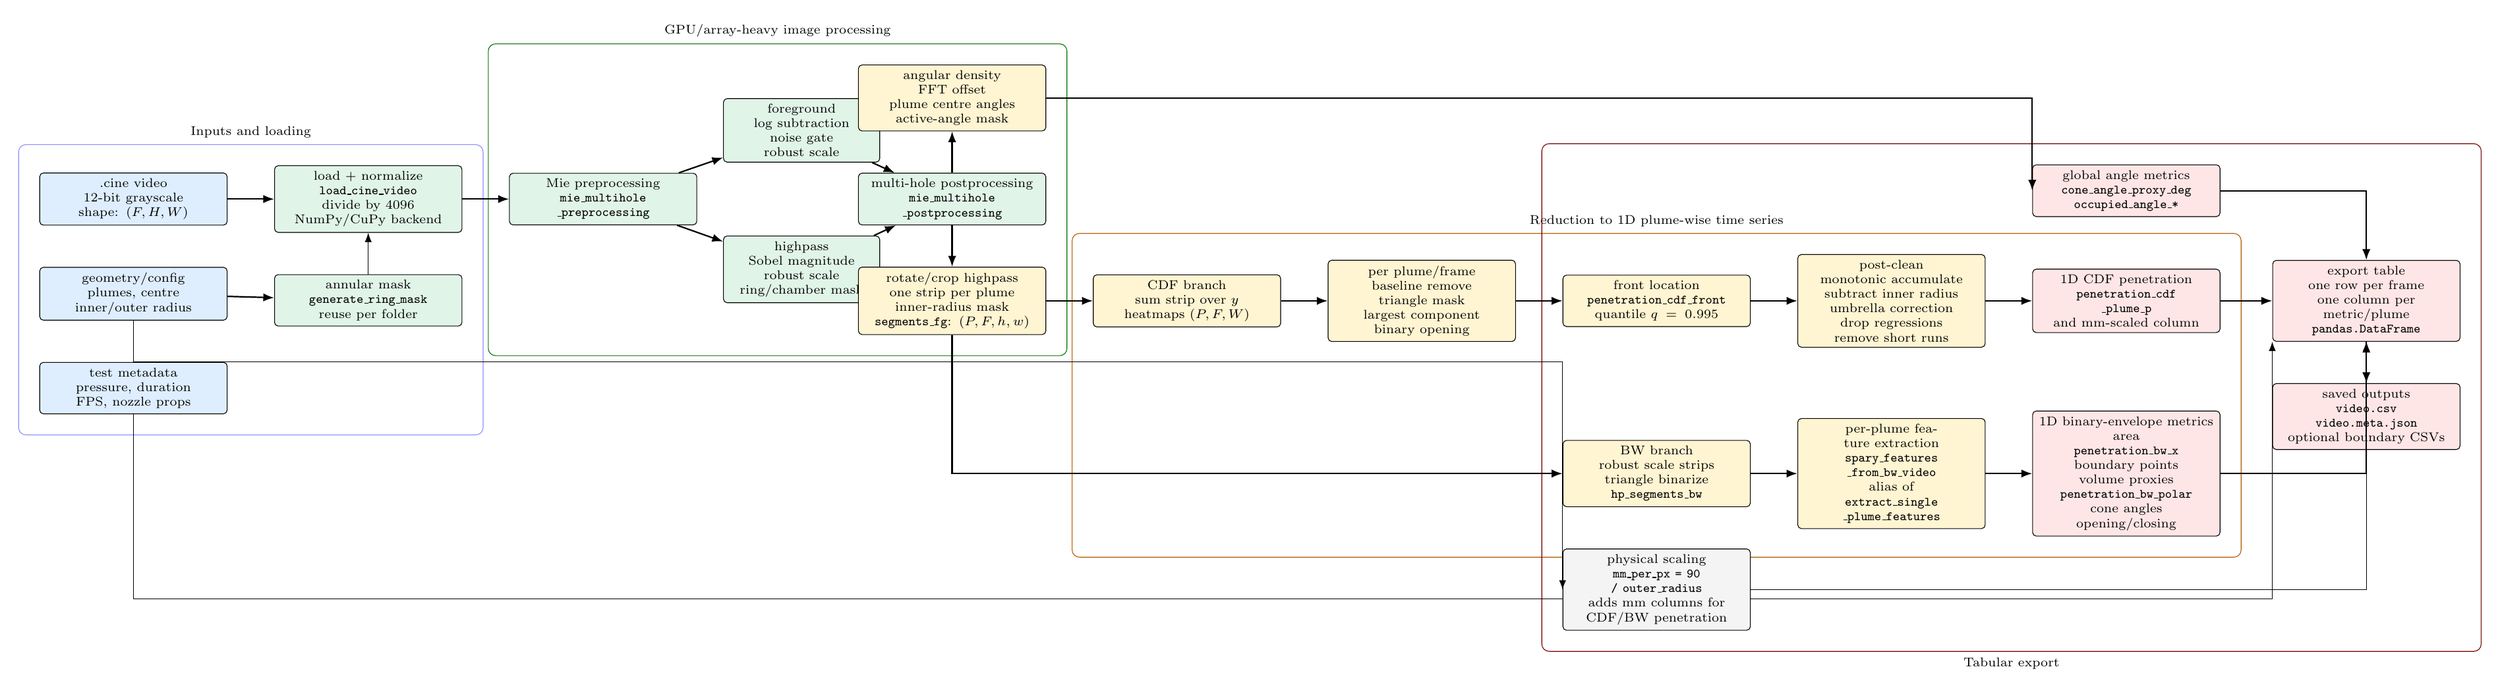
\begin{tikzpicture}[node distance=8mm and 9mm]

% Inputs and loading
\node[input] (cine) {.cine video\\12-bit grayscale\\shape: $(F,H,W)$};
\node[input, below=of cine] (cfg) {geometry/config\\plumes, centre\\inner/outer radius};
\node[input, below=of cfg] (meta) {test metadata\\pressure, duration\\FPS, nozzle props};

\node[process, right=of cine] (load) {load + normalize\\\texttt{load\_cine\_video}\\divide by 4096\\NumPy/CuPy backend};
\node[process, below=of load] (ring) {annular mask\\\texttt{generate\_ring\_mask}\\reuse per folder};

\draw[arrow] (cine) -- (load);
\draw[arrow] (cfg) -- (ring);
\draw[lightarrow] (ring) -- (load);

% Preprocess
\node[process, right=of load] (pre) {Mie preprocessing\\\texttt{mie\_multihole}\\\texttt{\_preprocessing}};
\node[smallbox, fill=processgreen, above right=2mm and 5mm of pre] (fg) {foreground\\log subtraction\\noise gate\\robust scale};
\node[smallbox, fill=processgreen, below right=2mm and 5mm of pre] (hp) {highpass\\Sobel magnitude\\robust scale\\ring/chamber mask};
\draw[arrow] (load) -- (pre);
\draw[arrow] (pre) -- (fg);
\draw[arrow] (pre) -- (hp);

% Postprocess
\node[process, right=31mm of pre] (post) {multi-hole postprocessing\\\texttt{mie\_multihole}\\\texttt{\_postprocessing}};
\node[branch, above=of post] (angle) {angular density\\FFT offset\\plume centre angles\\active-angle mask};
\node[branch, below=of post] (strip) {rotate/crop highpass\\one strip per plume\\inner-radius mask\\\texttt{segments\_fg}: $(P,F,h,w)$};
\draw[arrow] (fg) -- (post);
\draw[arrow] (hp) -- (post);
\draw[arrow] (post) -- (angle);
\draw[arrow] (post) -- (strip);

% Branch A CDF
\node[branch, right=of strip] (cdfprep) {CDF branch\\sum strip over $y$\\heatmaps $(P,F,W)$};
\node[branch, right=of cdfprep] (cdfclean) {per plume/frame\\baseline remove\\triangle mask\\largest component\\binary opening};
\node[branch, right=of cdfclean] (cdfx) {front location\\\texttt{penetration\_cdf\_front}\\quantile $q=0.995$};
\node[branch, right=of cdfx] (cdfpost) {post-clean\\monotonic accumulate\\subtract inner radius\\umbrella correction\\drop regressions\\remove short runs};
\node[output, right=of cdfpost] (cdfout) {1D CDF penetration\\\texttt{penetration\_cdf}\\\texttt{\_plume\_p}\\and mm-scaled column};
\draw[arrow] (strip) -- (cdfprep);
\draw[arrow] (cdfprep) -- (cdfclean);
\draw[arrow] (cdfclean) -- (cdfx);
\draw[arrow] (cdfx) -- (cdfpost);
\draw[arrow] (cdfpost) -- (cdfout);

% Global angle outputs
\node[output, above=10mm of cdfout] (globalmetrics) {global angle metrics\\\texttt{cone\_angle\_proxy\_deg}\\\texttt{occupied\_angle\_*}};
\draw[arrow] (angle.east) -| (globalmetrics.west);

% Branch B BW metrics
\node[output, below=15mm of cdfout] (bwout) {1D binary-envelope metrics\\area\\\texttt{penetration\_bw\_x}\\boundary points\\volume proxies\\\texttt{penetration\_bw\_polar}\\cone angles\\opening/closing};
\node[branch, left=of bwout] (features) {per-plume feature extraction\\\texttt{spary\_features}\\\texttt{\_from\_bw\_video}\\alias of\\\texttt{extract\_single}\\\texttt{\_plume\_features}};
\node[branch, left=of features] (bw) {BW branch\\robust scale strips\\triangle binarize\\\texttt{hp\_segments\_bw}};
\draw[arrow] (strip.south) |- (bw.west);
\draw[arrow] (bw) -- (features);
\draw[arrow] (features) -- (bwout);

% Export
\node[output, right=10mm of cdfout] (df) {export table\\one row per frame\\one column per metric/plume\\\texttt{pandas.DataFrame}};
\node[output, below=of df] (files) {saved outputs\\\texttt{video.csv}\\\texttt{video.meta.json}\\optional boundary CSVs};
\draw[arrow] (cdfout.east) -- (df.west);
\draw[arrow] (bwout.east) -| (df.south);
\draw[arrow] (globalmetrics.east) -| (df.north);
\draw[lightarrow] (meta.south) |- ([yshift=-12mm]bwout.south) -| (df.south west);
\draw[arrow] (df) -- (files);

% Metadata side note
\node[note, below=of bw] (scale) {physical scaling\\\texttt{mm\_per\_px = 90 / outer\_radius}\\adds mm columns for CDF/BW penetration};
\draw[lightarrow] (cfg.south) |- ([yshift=-8mm]cfg.south) -| (scale.west);
\draw[lightarrow] (scale.east) -| (df.south);

% Grouping backgrounds
\begin{scope}[on background layer]
  \node[draw=blue!45, rounded corners=4pt, fit=(cine)(cfg)(meta)(load)(ring), inner sep=4mm, label={[font=\scriptsize]above:Inputs and loading}] {};
  \node[draw=green!45!black, rounded corners=4pt, fit=(pre)(fg)(hp)(post)(angle)(strip), inner sep=4mm, label={[font=\scriptsize]above:GPU/array-heavy image processing}] {};
  \node[draw=orange!70!black, rounded corners=4pt, fit=(cdfprep)(cdfclean)(cdfx)(cdfpost)(cdfout)(bw)(features)(bwout), inner sep=4mm, label={[font=\scriptsize]above:Reduction to 1D plume-wise time series}] {};
  \node[draw=red!45!black, rounded corners=4pt, fit=(globalmetrics)(df)(files)(scale), inner sep=4mm, label={[font=\scriptsize]below:Tabular export}] {};
\end{scope}

\end{tikzpicture}%
}

\vfill
\scriptsize
Code anchors: \texttt{mie\_multi\_hole.py:\_process\_cine\_file}, \texttt{OSCC\_postprocessing.analysis.mie\_multihole}, and \texttt{OSCC\_postprocessing.binary\_ops.feature\_extraction}. The diagram shows the active pipeline from a normalized cine video to frame-wise 1D metrics; checkpointing and batch-folder traversal are omitted for clarity.

\newpage

\begin{center}
\Large\bfseries Fit Raw Data Pipeline: 1D Metrics to Curve Parameters
\end{center}

\vspace{-1mm}

\noindent\resizebox{0.98\linewidth}{!}{%
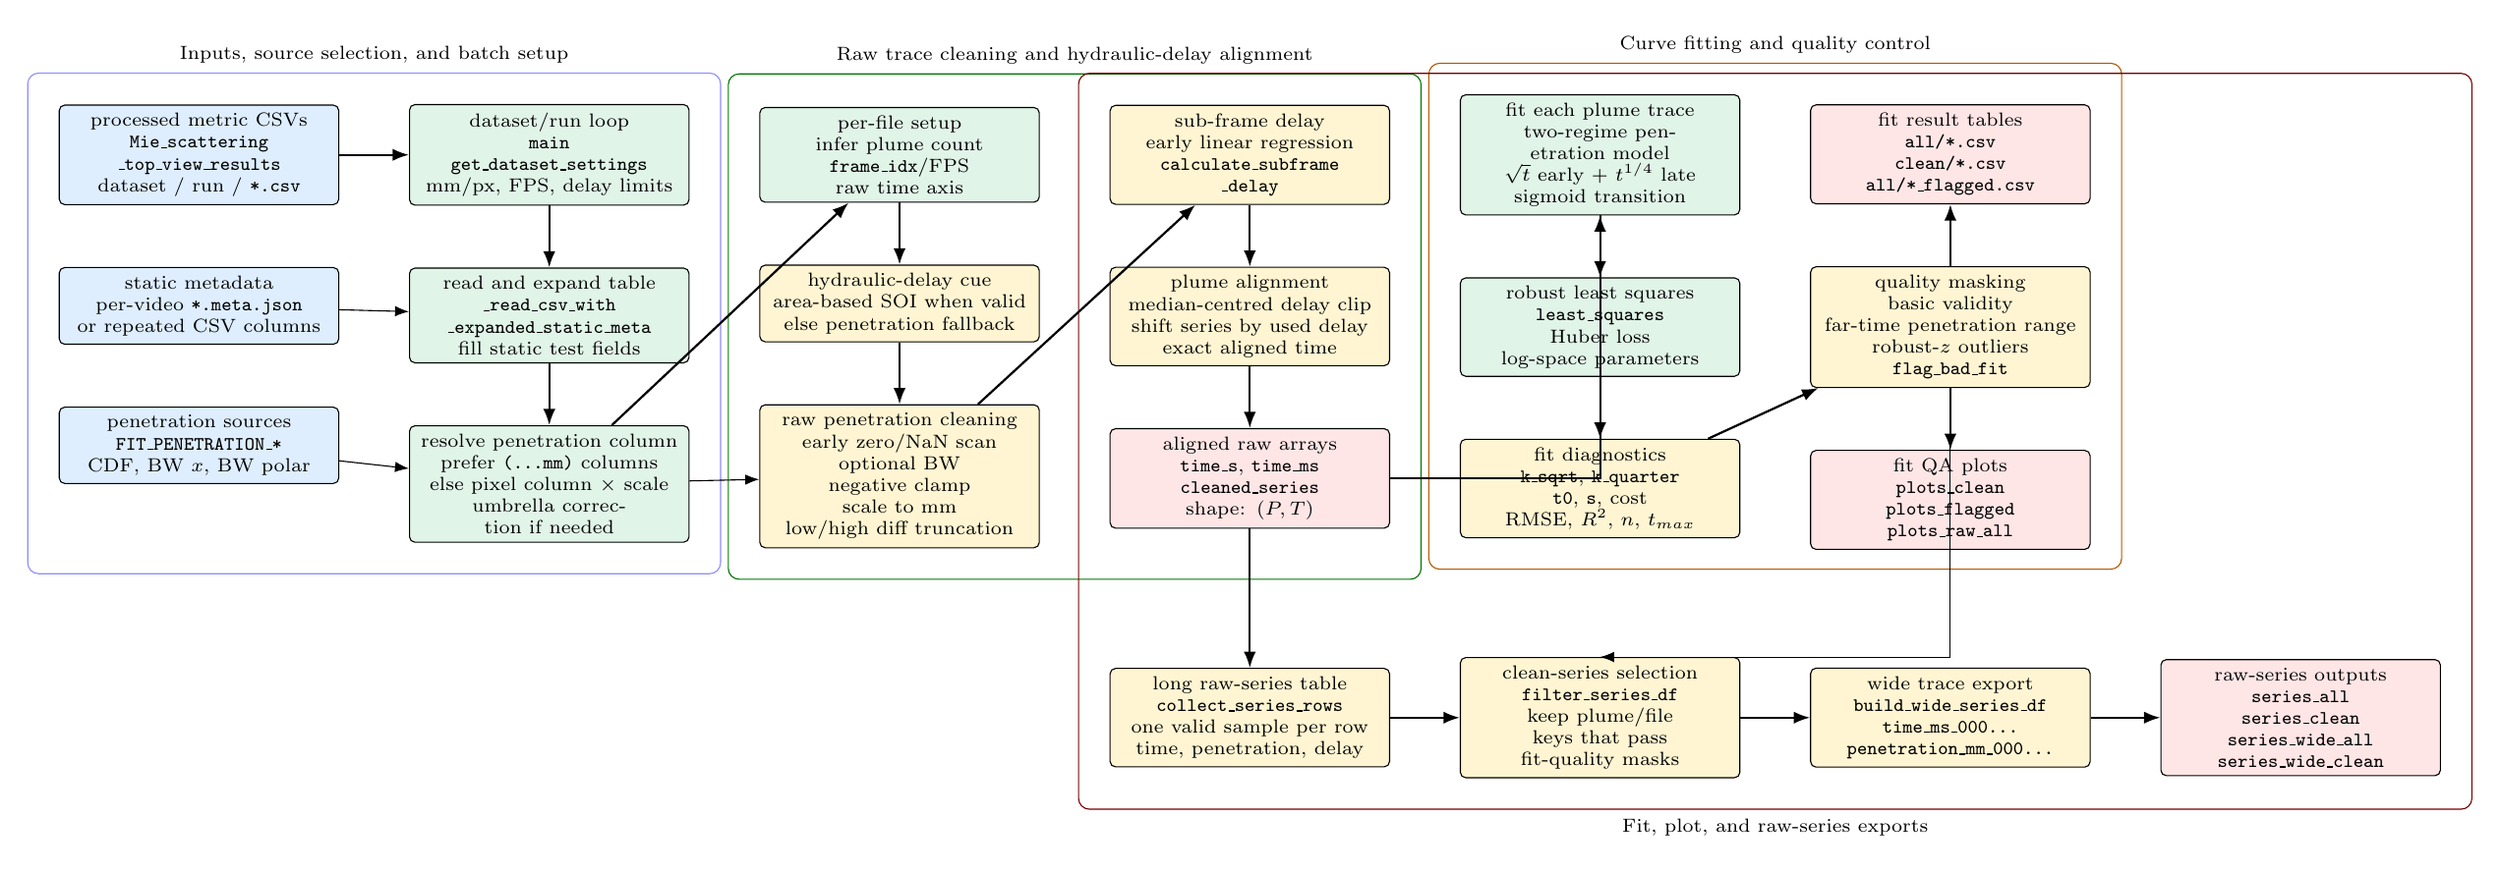
\begin{tikzpicture}[node distance=8mm and 9mm]

% Inputs and batch setup
\node[input] (csvs) {processed metric CSVs\\\texttt{Mie\_scattering}\\\texttt{\_top\_view\_results}\\dataset / run / \texttt{*.csv}};
\node[input, below=of csvs] (metajson) {static metadata\\per-video \texttt{*.meta.json}\\or repeated CSV columns};
\node[input, below=of metajson] (sources) {penetration sources\\\texttt{FIT\_PENETRATION\_*}\\CDF, BW $x$, BW polar};

\node[process, right=of csvs] (loop) {dataset/run loop\\\texttt{main}\\\texttt{get\_dataset\_settings}\\mm/px, FPS, delay limits};
\node[process, below=of loop] (read) {read and expand table\\\texttt{\_read\_csv\_with}\\\texttt{\_expanded\_static\_meta}\\fill static test fields};
\node[process, below=of read] (resolve) {resolve penetration column\\prefer \texttt{(...mm)} columns\\else pixel column $\times$ scale\\umbrella correction if needed};

\draw[arrow] (csvs) -- (loop);
\draw[arrow] (loop) -- (read);
\draw[lightarrow] (metajson) -- (read);
\draw[lightarrow] (sources) -- (resolve);
\draw[arrow] (read) -- (resolve);

% Per-file series preparation
\node[process, right=of loop] (axes) {per-file setup\\infer plume count\\\texttt{frame\_idx}/FPS\\raw time axis};
\node[branch, below=of axes] (delay) {hydraulic-delay cue\\area-based SOI when valid\\else penetration fallback};
\node[branch, below=of delay] (clean) {raw penetration cleaning\\early zero/NaN scan\\optional BW negative clamp\\scale to mm\\low/high diff truncation};

\draw[arrow] (resolve) -- (axes);
\draw[arrow] (axes) -- (delay);
\draw[arrow] (delay) -- (clean);
\draw[lightarrow] (resolve) -- (clean);

% Delay refinement and aligned arrays
\node[branch, right=of axes] (subdelay) {sub-frame delay\\early linear regression\\\texttt{calculate\_subframe}\\\texttt{\_delay}};
\node[branch, below=of subdelay] (align) {plume alignment\\median-centred delay clip\\shift series by used delay\\exact aligned time};
\node[output, below=of align] (aligned) {aligned raw arrays\\\texttt{time\_s}, \texttt{time\_ms}\\\texttt{cleaned\_series}\\shape: $(P,T)$};

\draw[arrow] (clean) -- (subdelay);
\draw[arrow] (subdelay) -- (align);
\draw[arrow] (align) -- (aligned);

% Fit branch
\node[process, right=of subdelay] (fitmodel) {fit each plume trace\\two-regime penetration model\\$\sqrt{t}$ early + $t^{1/4}$ late\\sigmoid transition};
\node[process, below=of fitmodel] (solver) {robust least squares\\\texttt{least\_squares}\\Huber loss\\log-space parameters};
\node[branch, below=of solver] (diagnostics) {fit diagnostics\\\texttt{k\_sqrt}, \texttt{k\_quarter}\\\texttt{t0}, \texttt{s}, cost\\RMSE, $R^2$, $n$, $t_{max}$};

\draw[arrow] (aligned) -| (fitmodel);
\draw[arrow] (fitmodel) -- (solver);
\draw[arrow] (solver) -- (diagnostics);

% Quality masking and fit outputs
\node[branch, right=of solver] (mask) {quality masking\\basic validity\\far-time penetration range\\robust-$z$ outliers\\\texttt{flag\_bad\_fit}};
\node[output, above=of mask] (fitcsv) {fit result tables\\\texttt{all/*.csv}\\\texttt{clean/*.csv}\\\texttt{all/*\_flagged.csv}};
\node[output, below=of mask] (plots) {fit QA plots\\\texttt{plots\_clean}\\\texttt{plots\_flagged}\\\texttt{plots\_raw\_all}};

\draw[arrow] (diagnostics) -- (mask);
\draw[arrow] (mask) -- (fitcsv);
\draw[arrow] (mask) -- (plots);

% Raw-series export branch
\node[branch, below=18mm of aligned] (seriesrows) {long raw-series table\\\texttt{collect\_series\_rows}\\one valid sample per row\\time, penetration, delay};
\node[branch, right=of seriesrows] (seriesclean) {clean-series selection\\\texttt{filter\_series\_df}\\keep plume/file keys that pass\\fit-quality masks};
\node[branch, right=of seriesclean] (wide) {wide trace export\\\texttt{build\_wide\_series\_df}\\\texttt{time\_ms\_000...}\\\texttt{penetration\_mm\_000...}};
\node[output, right=of wide] (seriesout) {raw-series outputs\\\texttt{series\_all}\\\texttt{series\_clean}\\\texttt{series\_wide\_all}\\\texttt{series\_wide\_clean}};

\draw[arrow] (aligned) -- (seriesrows);
\draw[arrow] (seriesrows) -- (seriesclean);
\draw[arrow] (seriesclean) -- (wide);
\draw[arrow] (wide) -- (seriesout);
\draw[lightarrow] (mask.south) |- (seriesclean.north);

% Grouping backgrounds
\begin{scope}[on background layer]
  \node[draw=blue!45, rounded corners=4pt, fit=(csvs)(metajson)(sources)(loop)(read)(resolve), inner sep=4mm, label={[font=\scriptsize]above:Inputs, source selection, and batch setup}] {};
  \node[draw=green!45!black, rounded corners=4pt, fit=(axes)(delay)(clean)(subdelay)(align)(aligned), inner sep=4mm, label={[font=\scriptsize]above:Raw trace cleaning and hydraulic-delay alignment}] {};
  \node[draw=orange!70!black, rounded corners=4pt, fit=(fitmodel)(solver)(diagnostics)(mask), inner sep=4mm, label={[font=\scriptsize]above:Curve fitting and quality control}] {};
  \node[draw=red!45!black, rounded corners=4pt, fit=(fitcsv)(plots)(seriesrows)(seriesclean)(wide)(seriesout), inner sep=4mm, label={[font=\scriptsize]below:Fit, plot, and raw-series exports}] {};
\end{scope}

\end{tikzpicture}%
}

\vfill
\scriptsize
Code anchors: \texttt{MLP/fit\_raw\_data.py:main}, \texttt{process\_folder}, \texttt{prepare\_cleaned\_series}, \texttt{fit\_sigmoid}, \texttt{apply\_filter\_masking}, \texttt{build\_wide\_series\_df}, and \texttt{save\_fit\_plot}. The diagram shows the per-penetration-source path from processed 1D plume metrics to fitted curve parameters, quality flags, QA plots, and raw-series exports.

\end{document}
